\section{Coding practice}

\subsection{Naming conventions}
\enumstart
	\item Goal: Consistency
	\item Consistency within an environment improves code readability
	\\ 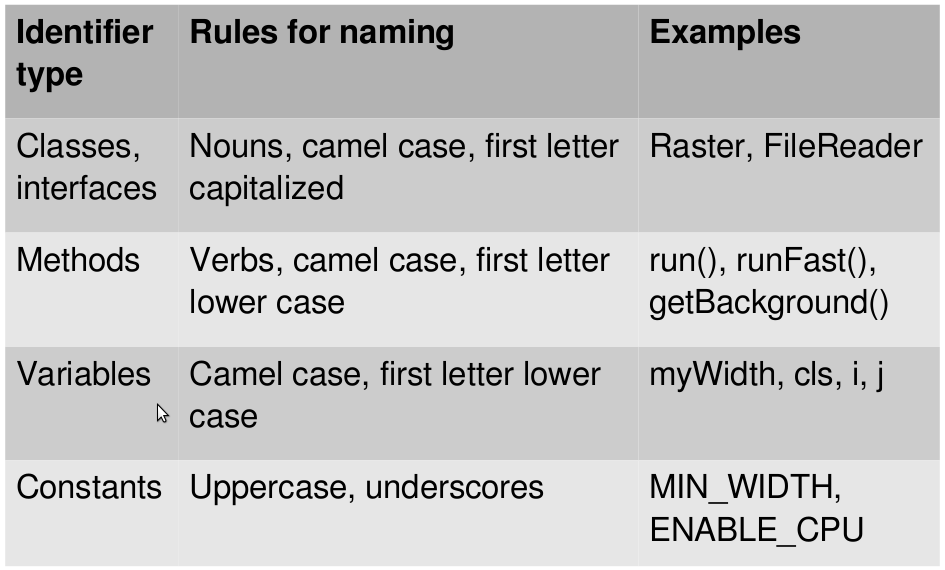
\includegraphics[width=0.5\textwidth]{img/java_naming_conventions.png}
	\item Method names
	\enumstart
		\item Goal: Help understand what a method does without inspecting its implementation
		\item Setters and getters of fields: getBlub(), setBla()
		\item Status methods: isFoo(), hasBar()
		\item Names that suggest side-effect freedom: findX()
		\item Names that suggest to have side-effects: openConnection()
	\enumend
	\item Longer names $\rightarrow$ better comprehension of source code
	\item But names can also be too long
\enumend

\subsection{Code Formatting}
\enumstart
	\item Consistent indentation
	\item Use spaces consistently
	\item Use brackets consistently
\enumend

\subsection{Documentation}
\enumstart
	\item API documentation
	\enumstart
		\item Help others to use your code without understanding its details
		\item Javadoc
	\enumend
	\item Code documentation
	\enumstart
		\item Ideally, the code makes clear what it does
		\item Comments should explain why you do it
	\enumend
\enumend

\subsection{Software clones}
\enumstart
	\item Copy-and-paste of source code fragments
	\item Take a working piece of code and reuse it by adapting it slightly
	\item Problem:
	\enumstart
		\item The same bug might occur multiple times
		\item Lines of code to maintain increase without adding new functionality
		\item When changing one clone, must change all clones, but cloning is not documented
	\enumend
	\item Solution:
	\enumstart
		\item Encapsulate reusable code into methods
		\item Replace clones by call to the reusable method
		\item Whenever you use copy-and-paste, think about other reuse mechanisms
	\enumend
\enumend

\subsection{Liskov's substitutability principle}
\enumstart
	\item A subclass instance used through the superclass type should behave like a superclass instance
	\item Bad Practice: Subclasses that reuse the superclass implementation but that do not semantically substitute the superclass
\enumend

\subsection{Test-driven development}
\enumstart
	\item Assumption that testing is a fundamental part of development
	\item Philosophy: Testing drives development
	\enumstart
		\item Testing doesn't occur after implementing
		\item Testing occurs before and during the implementation
	\enumend
	\item Result: increased confidence when changing code
	\item Steps
	\enumstart
		\item Add a test
		\item Run all tests and see the new one fail
		\item Change production code
		\item Run all tests and see them pass
	\enumend
	\item Philosophy: Production code is written to make failing tests pass
	\item How to test one class if other classes are still missing?
	\enumstart
		\item Create mock objects that simulate the behaviour of missing classes
		\item Same interface as real objects
		\item Simpler implementation (e.g. return default values)
		\item Also usefull if other classes exist but are difficult to integrate into a unit test
	\enumend
	\item How many tests do we need?
	\enumstart
		\item Testing cannot prove your program correct
		\item Should cover all functionality of the class under test
		\item Code coverage quantifies which percentage of your code is exercised by tests
	\enumend
\enumend

\subsection{Version-control}
\enumstart
	\item All software has different versions
	\enumstart
		\item Each time a developer changes the code
		\item Versions within the development cicle
		\item Versions for different platforms
	\enumend
	\item Why use version-control?
	\enumstart
		\item Allow more than one developer to work on the code
		\item Recreate old versions
		\item Change log
		\item Find who is responsible for a piece of code
	\enumend
\enumend
